\begin{figure*}[htbp]
    \centering
    \begin{tabular}{m{0.45\linewidth} m{0.45\linewidth} m{0.1\linewidth}}
        \begin{minipage}[b]{\linewidth}
            \centering
            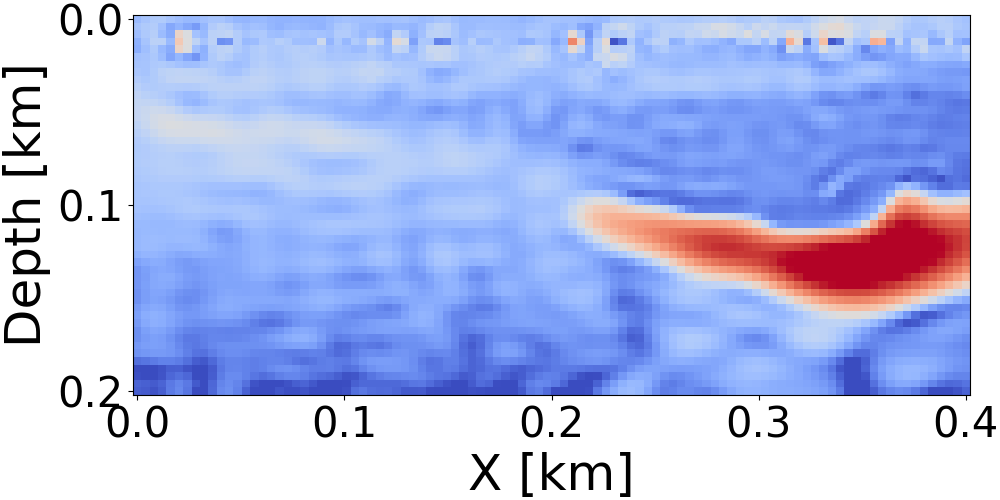
\includegraphics[width=\linewidth]{public/gradient_noisy}
            \caption*{(e) Standard FWI}
        \end{minipage} &
        \begin{minipage}[b]{\linewidth}
            \centering
            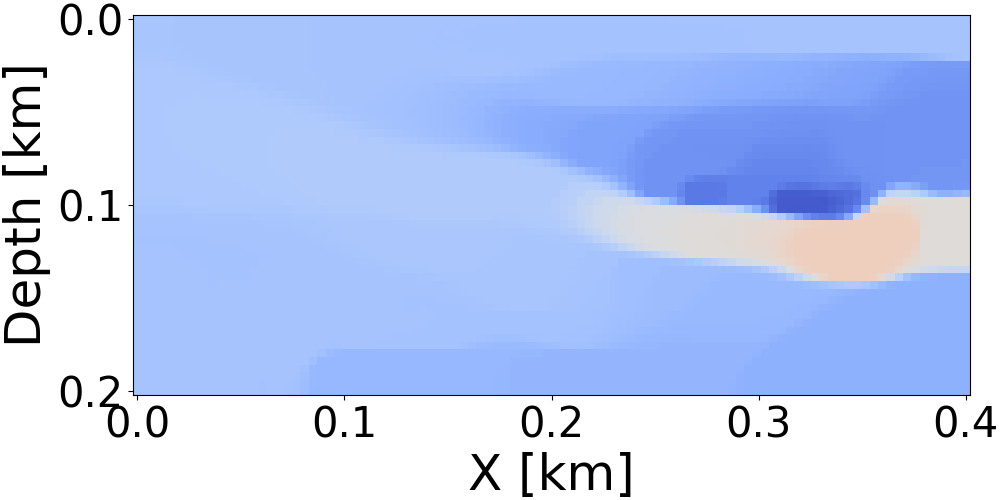
\includegraphics[width=\linewidth]{public/alpha_150_noisy}
            \caption*{(f) Proposed, $\alpha$ = 150}
        \end{minipage} &
        \multirow[t]{3}{*}{\raisebox{-51mm}{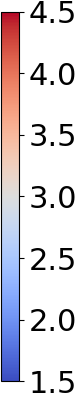
\includegraphics[height=50mm]{public/color-bar}}} \\

        \begin{minipage}[b]{\linewidth}
            \centering
            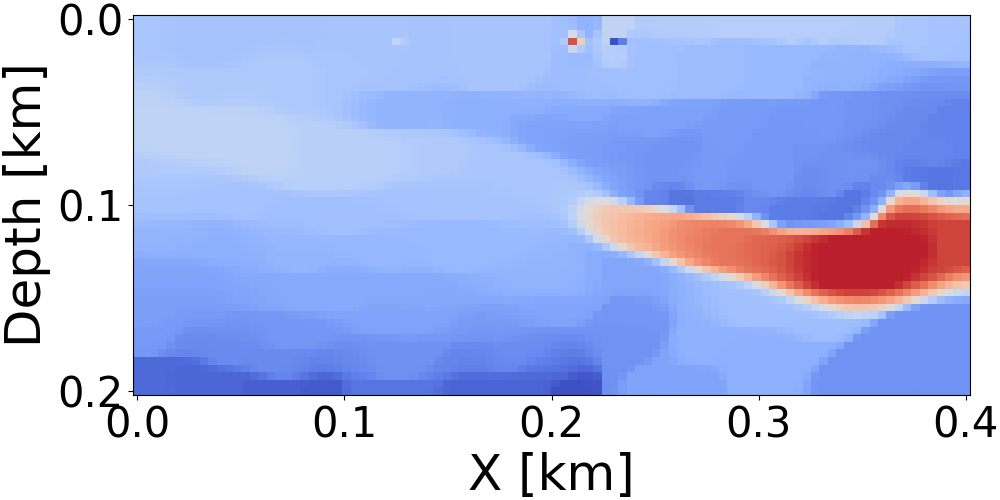
\includegraphics[width=\linewidth]{public/alpha_350_noisy}
            \caption*{(g) Proposed, $\alpha$ = 350}
        \end{minipage} &
        \begin{minipage}[b]{\linewidth}
            \centering
            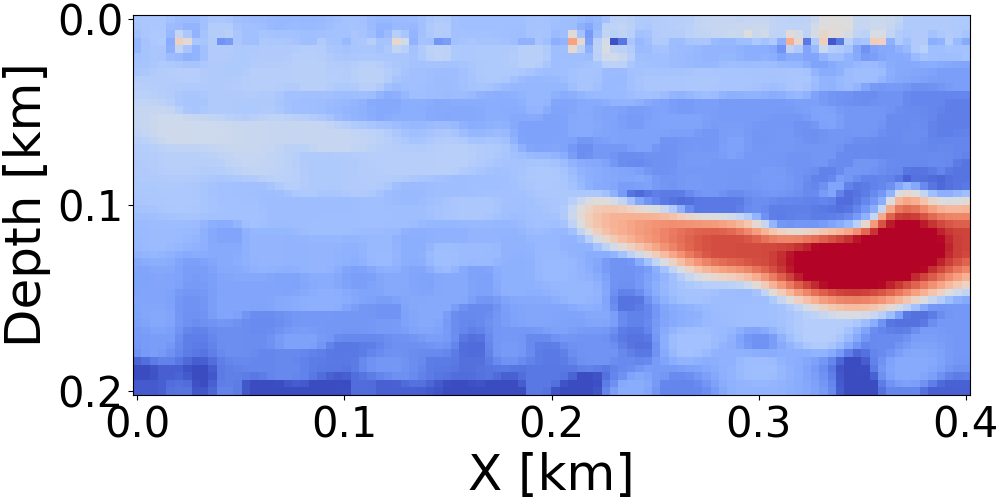
\includegraphics[width=\linewidth]{public/alpha_550_noisy}
            \caption*{(h) Proposed, $\alpha$ = 550}
        \end{minipage} &
    \end{tabular}
    \captionsetup{margin=1cm}
    \caption{
        Velocity models [km/s] and their corresponding reconstructions (with the noisy data). Similar to Fig.~\ref{fig:velocity-models-pure}, (g) is the best result, and (f)/(h) are the results with stronger/weaker TV constraint.
    }
    \label{fig:velocity-models-noisy}
\end{figure*}

